\section{Michelson Interferometer}
Das Michelson-Interferometer ist eines der bekanntesten
Messgeräte. Bekanntheit erlangte es durch das Michelson-Morley-Experiment, 
bei diesem Experiment sollte der Lichtäther untersucht werden.\\
Bei Michelson-Interferometer wird die optische Interferenz ausgenutzt, welche
nur bei kohärentem Licht beobachtet werden kann. Durch 
einen Strahlteiler wird der einfallende Lichtstrahl, meist
ein Laserstrahl, aufgespalten und diese Teilstrahlen interferieren anschließend
mit sich selbst.\\\\
\textbf{Prinzip des Michelson Interferometer:}\\
Wie oben bereits kurz erwähnt, teilt das Michelson-Interferometer
die Lichtwelle in zwei Teile auf. Diese Aufteilung geschieht 
mit einem Strahlteiler, einem halbdurchlässigen Spiegel. 
Der einfallende Lichtstrahl wird am Teiler zum Teil transmittiert 
und der restliche Teil des Strahls wird um 90° reflektiert. 
In unserem Fall beträgt der transmittierte und reflektierte Anteil 
jeweils 50\%.\\
Die beiden Teilstrahlen treffen jeweils auf einen total
reflektierenden Spiegel. Durch diese totale Reflexion
treffen die Strahlen erneut auf den Strahlteiler. Hier
wird wieder der eine Teil reflektiert und der andere 
transmittiert. Es kommt zu Überlagerung zweier Wellen 
hinter dem Strahlteiler. Die beiden Teilstrahlen müssen 
nicht die gleiche Strecke zurückgelegt haben. Durch 
beispielsweise Veränderung der Position einer der Spiegel kommt es zur 
Änderung der optischen Weglänge. Somit ergibt
sich eine Phasenverschiebung. Diese Verschiebung führt letzten Endes 
zur Interferenz, bei Addition der beiden Amplituden spricht man von
\textit{konstruktiver Interferenz} und bei Auslöschung der beiden 
Amplituden von \textit{destruktiver Interferenz}. 
Die Intensität kann nun gemessen werden und es 
können Rückschlüsse auf den Gangunterschied zwischen den beiden 
Wellen gezogen werden \citep[vgl.][]{Zusatzliteratur}.\\
Die folgende Grafik stellt einen schematischen Aufbau eines 
Michelson-Interferometer dar:
\begin{figure}[h]
    \centering
    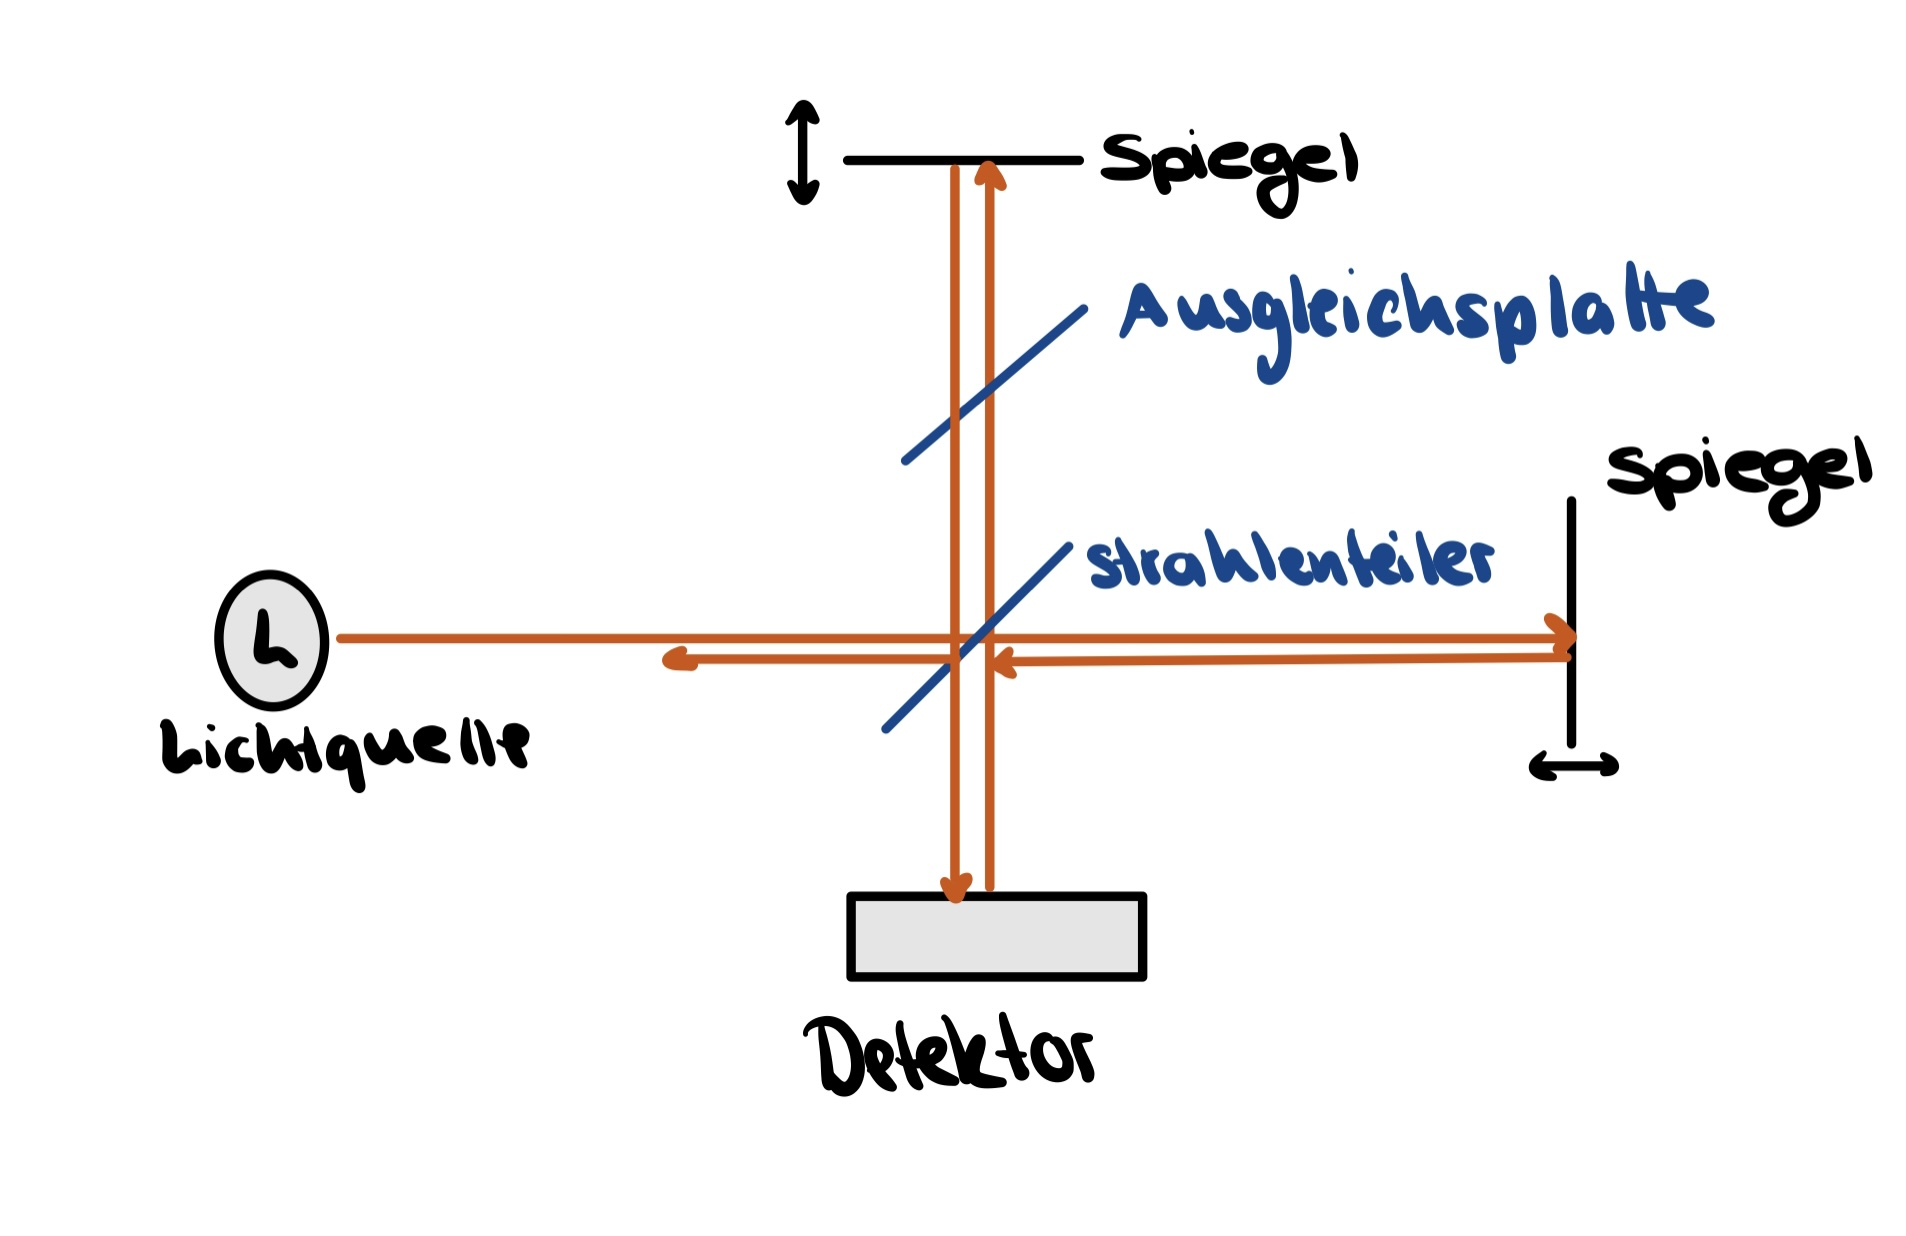
\includegraphics[width=0.6\textwidth]{FzV/michelson.jpg}
    \caption{Schematische Darstellung eines Michelson-Interferometer}
\end{figure}\newpage

\section{Ausgleichsplatte}
Wie oben bereits beschrieben durchlaufen die Teilstrahlen 
unterschiedlich oft auf den Strahlteiler. Der transmittierte Teilstrahl durchläuft dreimal 
und der reflektierte Strahl nur einmal den Strahlteiler. Um 
diese Ungleichheit zu bereinigen, wird eine Ausgleichsplatte 
zwischen den Strahlteiler und den total reflektierenden Spiegel 
des reflektierten Strahls gebaut. Hierbei ist es wichtig, 
dass die Ausgleichsplatte und der Strahlteiler die gleiche Dicke und Beschichtung
haben. Durch dieses zusätzliche Bauteil kommt es zu gleichen 
Absorption und Dispersion der zwei Teilstrahlen. \\
Würde die Ausgleichsplatte nicht eingebaut werden, wären die Interferometerarme
nicht dispersionsgleich. Dies hat zur Folge, dass es im Interferogramm zu einer
Phasenverschiebung ($\cos(kl)$ wird zu $\cos(kl+\phi)$) kommt.
Diese müsste erst bereinigt werden, damit man die richtigen Messwerte 
erhält und somit erschwert die Phasenverschiebung die Fourier Rücktransformation
erheblich. \citep[vgl.][]{Zusatzliteratur}

\section{Kohärenzlänge und Kohärenzzeit}
Als \textbf{Kohärenzlänge} $l_c$ bezeichnet man den maximal zulässigen 
Gangunterschied $\Delta s$, bei dem die Überlagerung zweier Lichtstrahlen (ausgesendet aus
derselben Quelle) noch ein stabiles Interferenzmuster ergibt. \\
Je mehr eine Lichtquelle monochromatisches Licht mit zeitlich konstanten
Polarisations- und Phasenbeziehung aussendet, umso größer ist die Kohärenzlänge.
Dies erklärt auch wieso Laser ein Licht mit großer Kohärenzlänge, d.h. im Bereich von 
Kilometern, aussenden und natürliche Quellen nur eine Kohärenzlänge im Bereich von wenigen $\mu m$ haben.\\
Die \textbf{Kohärenzzeit} $\tau_c$ ist die Zeit, in der 
das Licht die Kohärenzlänge zurücklegt:
\begin{equation*}
    \tau_c = \frac{n \cdot l_c}{c}
\end{equation*}
Hier steht n für den Brechungsindex des Mediums und c für 
die Lichtgeschwindigkeit. \\
Ein Anwendungsbeispiel für Kohärenzlänge ist das Zweistrahl
Interferometer. 
Wenn der Wert des Intensitätsmaximum der Interferenz 
$\frac{1}{\text{e}}$ beträgt, dann lässt sich die Kohärenzlänge 
mithilfe der halben Halbwertsbreite des Maximums und der Einhüllenden 
des Interferometers bestimmen. 
\citep[vgl.][]{wikik,Zusatzliteratur}
\newpage

\section{Fourier-Transformationsspektroskopie}
Das Fourier-Transformations-Spektrometer ist aus wenigen grundlegenden Bauteilen aufgebaut. 
Zum einen benötigt man eine Strahlungsquelle, einen Strahlengang (d.h. optische 
Anordnung von verschieden Spiegeln), Interferometer, Strahlungsdetektor und ein Messprogramm, 
welches die Fourier-Transformation durchführen kann. Zur Veranschaulichung ist der Versuchsaufbau
in der Abbildung \ref{fig:Versuch} zu sehen.\\
Nachdem die Strahlen das Michelson-Interferometer verlassen haben, interferieren diese, abhängig
von den Frequenzen bzw. der Differenz der Strahlen. Somit erhält man ein Interferogramm, 
welches ein großes Maximum vorweist, wenn die beiden Spiegel gleich weit von Strahlteiler 
entfernt sind. Ist dies der Fall so interferieren die Frequenzen konstruktiv.  
\begin{figure}[h]
    \centering
    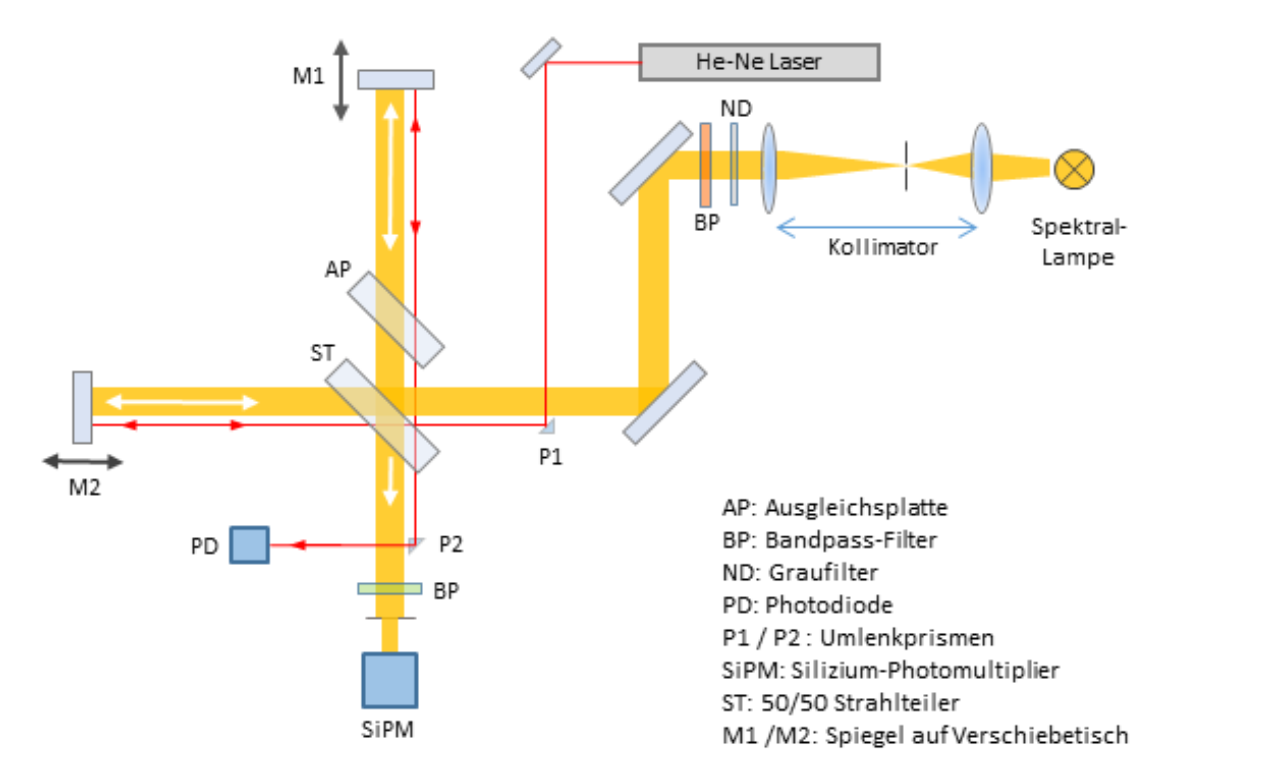
\includegraphics[scale=0.4]{FzV/Versuch.png}
    \caption{Schematische Darstellung des Versuchsaufbaus.}
    \label{fig:Versuch}
\end{figure}

\textbf{Vorteile von Fourier-Transformation-Spektrometern}\\
Ein großer Vorteil dieses Spektrometers ist, im Vergleich zu den Spektrometern, welche Monochromator 
verwenden, dass sich das Fourier-Transformation-Spektrometer durch eine deutlich kürzere Messzeit auszeichnet. Damit 
ist auch ein besseres Signal-Rausch-Verhältnis verbunden. Zudem ist es wie oben erwähnt aus 'einfacheren'
optischen Bauteilen aufgebaut und somit meist günstiger als etwaige Alternativen.\\
Des Weiteren gibt es noch den sogenannten \textit{Jacquinot-Vorteil:}\\
Bei einem dispersiven Spektrometer benötigt man einen Spaltblende, diese bestimmt 
im Wesentlichen die Auflösung des Spektrometers. Durch diese Blende kann es 
auch zu Beugungserscheinungen kommen. Diese ist bei einem
Fourier-Transformation-Spektrometer nicht mehr notwendig, es können auch Kreisblenden verwendet werden. 
Diese Blenden haben den Vorteil, dass mehr Licht den Detektor erreicht und sie 
somit ebenfalls das Signal-Rausch-Verhältnis verbessert.\\
Es gibt noch den \textit{Multiplex- oder Fellgett-Vorteil:}\\
Bei der Fouriertransformierten-Spektroskopie wird ein Interferometer anstatt eines dispersiven Spektrometern verwendet.
Hierbei wird das Spektrum nicht kontinuierlich in Abhängigkeit von der Wellenlänge gemessen, 
sondern beinahe alle Wellenlängen gleichzeitig.
Es wird quasi eine Momentaufnahme über den definierten Frequenzbereich gemacht. 
Dies wird v. a. bei sogenannten 
Fast-Scanning Fourier-Transformation-Spektrometern verwendet, hierdurch können Aufnahmezeiten 
von wenigen Sekunden erreicht werden.
Auch hierdurch kommt es ebenfalls zu einer Verbesserung des Signal-Rausch-Verhältnis.\\
Zuletzt soll noch der \textit{Connes-Vorteil} diskutiert werden:\\
Bei der Fouriertransformierten-Spektroskopie wird ein Helium-Neon-Laser verwendet. 
Durch diesen Referenzpunkt erhält man eine hohe Genauigkeit bei 
der Frequenz- bzw. Wellenlängenachse. \citep[vgl.][]{wikiFTIR, Zusatzliteratur}

\section{Faltungsprodukt und Autokorrelationsfunktion}
\subsection{Faltungsprodukt}
Die Faltung ist allgemein wie folgt definiert:
\begin{equation}
    f * g = \int_{- \infty}^{\infty} f(x-t) g(t) dt
\end{equation}
Wenn man dies jedoch Fourier transformiert, wird hieraus das Produkt der Fouriertransformierten der einzelnen Funktionen:
\begin{equation}
    F(f * g) = F(f) \cdot F(g)
\end{equation}
\citep[vgl.][]{Zusatzliteratur} 

\subsection{Autokorrelationsfunktion}
Die Autokorrelation ist ein Begriff aus der Signalverarbeitung. 
Diese beschreibt die Korrelation einer Funktion (bzw. Signals) mit sich 
selbst zu einem früheren Zeitpunkt. 
Mit der Autokorrelation ist es möglich, einen Zusammenhang 
zwischen Ereignissen einer Messreihe herzustellen, welche zu unterschiedlichen
Zeitpunkten stattfanden. \\
In der Signalverarbeitung wird sie als Faltung eines 
zeitabhängigen Signals $x(t)$ mit sich selbst berechnet.\\
In der digitalen Analyse von Signalen wird die Autokorrelationsfunktion
meistens über die inverse Fourier-Transformation der 
spektralen Leistungsdichte berechnet.\\
Ein Anwendungsbeispiel ist das Weißlichtintererometer:
Hier weicht die Autokorrelation deutlich von Null ab (bei geringer Kohärenzlänge), wenn 
die Länge von Messarm und Referenzarm gut übereinstimmen.
\citep[vgl.][]{Zusatzliteratur}


